\section{功的定义与作用点位移}

冲量把力沿时间累积，功则把力沿作用点的位移累积。对质点的一小段位移$\dd\bm r$，力$\bm F$做的元功为$\dd W=\bm F\cdot\dd\bm r$，全过程为$W=\int_A^B\bm F\cdot\dd\bm r$。恒力时才可直接化成$W=\bm F\cdot(\bm r_B-\bm r_A)$。正负由点积决定：沿位移的力分量做正功，反向分量做负功，垂直分量不做功。一个力可以做负功而另一个力做更大的正功，因此不能把某个力的功与合力总功混为一谈。

这里的位移必须是所用惯性参考系中受力作用点的位移。对于质点，作用点与质点位置相同；对于绳、滑轮和可变形物体，就要具体辨认作用点。把物块的位移代入拉绳自由端的拉力功，通常会漏掉滑轮传动的长度倍数。静止地面上的人起跳时，脚与地面接触处不动，地面支持力虽改变人体总动量，却不直接向人体输入机械功；肌肉消耗的化学能提供人体增加的机械能。相反，弹性跳板的接触点会移动，跳板可以对人做功。

若$\bm F$随位置变化，可以选坐标直接积分。例如沿$x$方向的力$F_x(x)$做功为$\int F_x\dd x$，对应$F_x-x$图线下的有向面积。曲线路径中也可取弧长$s$，只积切向分量$F_t$：$W=\int F_t\dd s$。不要把力的大小不加投影地乘路径长度；这只有力始终沿路径时才成立。

\fig{fig:em3:work}{元功中的切向分量与作用点位移}{\begin{tikzpicture}[scale=.9]\draw[world,domain=0:3,samples=50]plot(\x,{.15*\x*\x});\coordinate(P)at(1.6,.384);\fill(P)circle(.05)node[below]{$P$};\draw[flow](P)--(3,1.056)node[right]{$\dd\bm r$};\draw[force](P)--(2.6,1.984)node[above]{$\bm F$};\draw[guide](2.6,1.984)--(3.037,1.074);\node at(.4,1.6){$\dd W=F_t\dd s$};\end{tikzpicture}}

图\ref{fig:em3:work}中的位移微元沿真实路径切线，只有力在该方向的投影进入元功。法向分量能使速度转向，却在这一瞬间不贡献功；位移还须取力的作用点，而非任意选取物体上另一点的位移。


\fig{fig:em3:moving-track}{支持力垂直相对运动方向，却一般不垂直受力点的对地速度}{\begin{tikzpicture}

\draw[world](0,0)--(4,0)--(4,2)--cycle;\fill(2,1)circle(2pt)node[below]{$P$};
\draw[force,red](2,1)--(1.4,2.2)node[above]{$\bm N$};
\draw[flow,blue](2,1)--(3,1.5)node[above]{$\bm v_{\text{相}}$};\draw[flow](2,1)--(4,1.5)node[right]{$\bm v$};
\draw[guide](3,1.5)--(4,1.5);\draw[flow,blue](1,-.7)--(2.4,-.7)node[right]{$\bm V_{\text{槽}}$};
\node at(2,3){$\bm v=\bm V_{\text{槽}}+\bm v_{\text{相}}$};

\end{tikzpicture}}
图\ref{fig:em3:moving-track}的斜槽向右平移，球的相对速度沿槽面。红色支持力指向左上，它与$\bm v_{\text{相}}$垂直，却与对地速度$\bm v$不垂直。这一图示中支持力对球做负功，同时对槽做等量正功；应根据所选对象分别列功。


在运动的约束面上，“垂直约束面”也不保证不做功。设光滑槽对球的支持力为$\bm N$，球对地速度为$\bm v=\bm V_{\text{槽}}+\bm v_{\text{相}}$，相对速度沿槽切线，因此$\bm N\cdot\bm v_{\text{相}}=0$，但对地功率为$\bm N\cdot\bm V_{\text{槽}}$，一般不为零。若把球与槽取为整体，两者在接触处的内力总功率才因无相对法向运动而相消。决定是否做功的是受力点在所选参考系中的真实速度。

\section{功与冲量为什么不能互相替代}

冲量是对时间的积分，功是对作用点位移的积分，二者不能直接互相替代。固定光滑墙使球以原速率反弹时，墙的法向冲量非零，但全过程净功为零；速度方向改变，速率不变。

反过来，某一个力也可以冲量相消而总功不为零。例如图\ref{fig:em3:friction-return}中，外部驱动使滑块以相同速率、等长时间往返，滑动摩擦在两段的方向相反，冲量相消，但两段都做负功。这里有外部驱动力，不能把摩擦力误当合力。
\fig{fig:em3:friction-return}{受外部驱动的等时往返中，摩擦冲量相消，摩擦功仍相加}{\begin{tikzpicture}

\foreach \yy in {1.8,0}{\draw[world](-1,\yy)--(5,\yy);\draw[world](1,\yy)rectangle(2,\yy+.6);}
\draw[flow,blue](1.2,3)--(2.5,3)node[right]{$u$};\draw[force,red](1.5,2.1)--(.2,2.1)node[left]{$f$};
\draw[flow,blue](1.8,1.2)--(.5,1.2)node[left]{$u$};\draw[force,red](1.5,.3)--(2.8,.3)node[right]{$f$};
\node[align=left]at(6.5,2){每段持续$\tau$\\$I_f=-f\tau+f\tau=0$};
\node[align=left]at(6.5,.2){两段位移与摩擦反向\\$W_f=-fu\tau-fu\tau<0$};

\end{tikzpicture}}
对恒质量质点，若说的是合外冲量为零，则始末速度矢量相同，动能也相同，合力总功必为零。区分“某个力”与“合力”，才不会把两个定理的适用对象混淆。


对恒质量质点，若合力与速度垂直，瞬时功率为零，速率不变，但方向可以持续改变。匀速圆周运动的向心力便如此。若某一力方向固定且物体沿该方向运动，已知全过程冲量可给出末速度，再由动能定理得到合力功；这里不是冲量等于功，而是借助同一初、末状态把两者联系起来。若还有其他力做功，求某一个力的功时仍需把其他项分开。

功的正负与参考系有关，但受力规律并不会矛盾。站在运动传送带旁观察，一个被摩擦加速的物块动能增加；在与带共速的惯性系中，物块的相对速率减小。相应摩擦力作用点的位移也改变，所以功一起改变。对块和带组成的系统，摩擦耗散仍由相对滑程确定，与这种匀速参考系变化无关。

\section{动能定理的推导与对象}

对恒质量质点，牛顿第二定律为$m\dd\bm v/\dd t=\bm F_{\text{合}}$。两边点乘$\bm v\dd t=\dd\bm r$，得到 $\bm F_{\text{合}}\cdot\dd\bm r=m\bm v\cdot\dd\bm v$。
这里 $v^2=\bm v\cdot\bm v$，乘积微分给
$\dd(v^2)=\dd\bm v\cdot\bm v+\bm v\cdot\dd\bm v=2\bm v\cdot\dd\bm v$。
因此沿实际路径从状态 $A$ 积到 $B$，
\[
\int_A^B\bm F_{\text{合}}\cdot\dd\bm r
=\int_{v_A^2}^{v_B^2}\frac m2\,\dd q
=\left[\frac m2q\right]_{v_A^2}^{v_B^2}
=\frac12mv_B^2-\frac12mv_A^2.
\]
记 $q=v^2$，便得到
\begin{equation}W_{\text{合}}=K_B-K_A,\qquad K=\frac12mv^2.\label{eq:em3:workenergy}\end{equation}
这一推导既适用于直线运动也适用于曲线运动。法向力改变速度方向，却不改变速率；在固定光滑轨道中，支持力垂直瞬时速度，不做功。若轨道本身移动，支持力相对地面的作用点可能有沿力方向的位移，此时不能继续断言它不做功。

对系统逐个质点求和，$\Delta K_\Sigma=W_{\text{外}}+W_{\text{内}}$，其中内力总功不能仅凭“成对”便删去。两力大小相等、方向相反，只保证冲量在总动量式中抵消；功还乘各自作用点的位移，若两作用点位移不同，总功未必为零。将系统划分为物块、木板或弹簧时，必须同步改变功的分类，不能在一个系统中把弹力功计入，另一个系统又把弹性势能重复计入。

\fig{fig:em3:internal-work}{弹簧推开两物体时，两内力冲量相消，但各自都能做正功}{\begin{tikzpicture}

\draw[world](0,0)rectangle(1,.8);\draw[world](3.5,0)rectangle(4.5,.8);\draw[spring](1,.4)--(3.5,.4);
\node at(.5,.4){$m_1$};\node at(4,.4){$m_2$};\draw[guide](2.3,-.7)--(2.3,2.4)node[above]{$X_C$固定};
\draw[force,red](.5,1.3)--(-.7,1.3)node[left]{$\bm F_1$};\draw[force,red](4,1.3)--(5.2,1.3)node[right]{$\bm F_2$};
\draw[flow,blue](.5,-.6)--(-.5,-.6)node[left]{$\dd\bm r_1$};\draw[flow,blue](4,-.6)--(5,-.6)node[right]{$\dd\bm r_2$};
\node at(2.2,-1.4){$\dd W_{\text{内}}=\bm F_1\cdot(\dd\bm r_1-\dd\bm r_2)>0$};

\end{tikzpicture}}
图\ref{fig:em3:internal-work}从整体静止开始，弹簧对两物体的力等大反向，但位移也相反，所以两个功都为正。弹性储能转为两物体的动能，而质心水平位置保持不变。总动量方程中可消去的内力，不能直接从总动能方程中删去。


若只想用合外力对质心位移的积分，应由$M\dd\bm V_C/\dd t=\bm F_{\text{外}}$得到
\[\Delta(MV_C^2/2)=\int\bm F_{\text{外}}\cdot\dd\bm R_C.\]
它描述的是质心平动动能，而不一定是系统总动能。例如两个物体被弹簧从静止推开，质心不动、合外力不做质心功，但系统总动能增加。因此系统题中要明确所写的$K$究竟包含哪些运动。

\section{变力积分与弹簧做功}

理想弹簧相对自然长的有符号伸长量为$x$，弹力为$-kx$，所以从$x_1$到$x_2$弹力所做的功为
\[
W_s=-k\int_{x_1}^{x_2}x\dd x
=-k[x^2/2]_{x_1}^{x_2}
=\frac12kx_1^2-\frac12kx_2^2.
\]
压缩和伸长均由平方量描述储能，但运动方向和接触条件仍须另外判断。弹簧只推动未连接的物块时，伸长后就不能继续把物块拉回来；若物块与弹簧连接，才可在自然长另一侧继续运动。

\fig{fig:em3:spring-area}{弹力关于有符号形变量的图线，压缩恢复与继续拉长的功具有相反符号}{\begin{tikzpicture}

\draw[axis](-2.5,0)--(2,0)node[right]{$x$};\draw[axis](0,-1.7)--(0,2.5)node[above]{$F_s$};
\fill[blue!15](-1.6,0)--(-1.6,1.6)--(0,0)--cycle;\fill[red!15](0,0)--(.9,-.9)--(.9,0)--cycle;
\draw[world,blue](-2,2)--(1.4,-1.4);\draw[guide](-1.6,0)--(-1.6,1.6);\draw[guide](.9,0)--(.9,-.9);
\node[below left]at(-1.6,0){$x_1<0$};\node[above right]at(.9,0){$x_2>0$};\node[right]at(1.1,-1.1){$F_s=-kx$};
\draw[flow](-1.6,2.3)--(-.2,2.3)node[midway,above]{从压缩恢复};

\end{tikzpicture}}
图\ref{fig:em3:spring-area}从$x_1<0$运动到$x_2>0$，先积蓝色正面积，再积红色负面积。两部分的有向和给$W_s=k(x_1^2-x_2^2)/2$。若物块只是顶在弹簧上而没有连接，运动到$x=0$便分离，红色部分不属于它的真实过程。


对于准静态过程，速度可近似为零，但力并不为零。外力逐点平衡其他力，外力功可由位移积分，也可从初、末势能差求出。积分时应说明所选变量怎样对应物体位移；浮力压沉问题中，液面也可能上升，浸入深度不等于木块下降距离。先写几何和体积关系，再把外力表示成同一积分变量的函数。

选积分变量时，应使力和作用点位移都能由同一变量表示。若阻力随总进入深度$x$增加，第二次推动的积分下限应是第一次已经达到的$d$，而不是重新从零起算。若沿圆弧用角度$\theta$积分，应先代入$\dd s=R\dd\theta$；若液面随压入距离$s$上升，应先用体积守恒把浸深写成$s$的函数，再把浮力代入功积分。漏掉变量之间的几何联系，往往比积分运算本身更容易造成错误。

\fig{fig:em3:float-coordinate}{木块下降与液面上升共同增加浸深，外力功须对木块下降量积分}{\begin{tikzpicture}

\foreach \sh/\level/\bot/\top in {0/2/1/3,6/2.2/.4/2.4}{
\begin{scope}[xshift=\sh cm]
\draw[world](0,3.5)--(0,0)--(4,0)--(4,3.5);\fill[blue!10](0,0)rectangle(4,\level);
\draw[fill=white](1.5,\bot)rectangle(2.5,\top);\draw[world,blue](0,\level)--(1.5,\level);\draw[world,blue](2.5,\level)--(4,\level);
\end{scope}}
\draw[dim](3,1)--(3,2)node[midway,right]{$d_0$};\node at(2,-.6){初始漂浮};
\draw[guide](6,2)--(10,2);\draw[guide](8.5,3)--(9.4,3);\draw[dim](9.2,2.4)--(9.2,3)node[midway,right]{$s$};
\draw[dim](10.5,2)--(10.5,2.2)node[right]{$\Delta h$};\draw[dim](7,.4)--(7,2.2)node[midway,left]{$d$};
\draw[force,red](8,3.6)--(8,2.5)node[pos=0,above]{$F$};\node at(8,-.6){容器面积$A$，木块截面积$a$};

\end{tikzpicture}}
图\ref{fig:em3:float-coordinate}取直壁容器和等截面木块、无溢流。木块下降$s$、液面上升$\Delta h$，浸深成为$d=d_0+s+\Delta h$。水体积守恒给$A\Delta h=a(s+\Delta h)$，所以
\[
d-d_0=\frac{A}{A-a}s,\qquad
F=B-mg=\rho ga\frac{A}{A-a}s.
\]
准静态压入所需外力向下，与木块位移同向，故在仍部分浸没的范围内
\[
W_{\rm ext}=\int_0^s F(s')\dd s'
=\frac{\rho gaA}{A-a}\left[\frac{s'^2}{2}\right]_0^s
=\frac{\rho gaA}{2(A-a)}s^2.
\]
积分变量是受力木块的下降距离$s'$，不是浸深$d$。完全浸没、触底或溢流之后，须按新边界另列方程。


\section{理想约束的内力总功}

两质点之间用不可伸长轻杆相连，令沿杆单位矢量为$\bm n$，两端内力为$T\bm n$与$-T\bm n$。其瞬时总功率是$T\bm n\cdot(\bm v_A-\bm v_B)$。杆长不变给$(\bm v_A-\bm v_B)\cdot\bm n=0$，所以内力总功率为零。这里每一端所受力可以单独做功，只是总和为零；若杆的某端固定，也可能两端分别都不做功。

若改成弹簧，两端沿弹簧方向的相对速度可以非零，内力总功率等于弹性势能变化率的负值。若改成滑动摩擦，内力总功率为$-f|v_{A,\text{切}}-v_{B,\text{切}}|$，对应耗散。三种情形的区别来自动力学与几何约束，而不是“内力”这个名称。判断系统机械能是否守恒，必须看相对运动与储能，不能只看力是否成对。

\fig{fv:e3:power}{同一杆内力可以分别做功，总功率由沿杆相对速度决定}{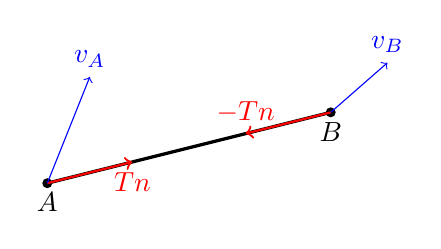
\begin{tikzpicture}[scale=.9]
\coordinate(A)at(0,0);\coordinate(B)at(4,1);\draw[very thick](A)--(B);\fill(A)circle(2pt)node[below]{$A$};\fill(B)circle(2pt)node[below]{$B$};
\draw[->,red,thick](A)--(1.2,.3)node[below]{$T\bm n$};\draw[->,red,thick](B)--(2.8,.7)node[above]{$-T\bm n$};
\draw[->,blue](A)--(.6,1.5)node[above]{$\bm v_A$};\draw[->,blue](B)--(4.8,1.7)node[above]{$\bm v_B$};
\end{tikzpicture}}
图\ref{fv:e3:power}的杆长条件限制的是 $(\bm v_A-\bm v_B)\cdot\bm n=0$。两端内力的总功率因而为零，尽管各自与端点速度的点积不必为零。若杆可伸长，这个投影一般不再为零，内力便可改变弹性储能。讨论“内力是否做功”之前，必须先明确说的是某一端的功，还是整个固定物质系统内力的总功。


\section{功率与速度传动}

瞬时功率为$P=\dd W/\dd t=\bm F\cdot\bm v_{\text{作用点}}$。恒定拉力不意味着恒功率，因为受力点的速度可能改变；匀速也不意味着功率为零，因为推力可以持续补偿摩擦耗散。对无质量、无摩擦的理想绳轮装置，可以用绳长约束求自由端速度，再算外拉力的功率，也可以把各段绳对被拉物体的合力与物体速度点乘。两条路线应给出相同结果。

\fig{fig:em3:pulley-power}{绳长约束使自由端速度为动滑轮速度的两倍，两端功率计算一致}{\begin{tikzpicture}

\draw[world](-.5,3)--(.5,3);\draw[world](0,3)--(0,1)arc(180:360:1)--(2,3.4);
\draw[world](1,1)circle(1);\fill(1,1)circle(2pt);\draw[world](1,1)--(1,-.8);\draw[world](.5,-1.5)rectangle(1.5,-.8);\node at(1,-1.15){$M$};
\draw[flow,blue](3,2)--(3,3.2)node[above]{$v_{\text{端}}=2v$};\draw[force,red](2,3.4)--(2,4.3)node[above]{$F$};
\draw[flow,blue](3,-1.2)--(3,0)node[above]{$v$};
\draw[force](0,1)--(0,2.2)node[left]{$F$};\draw[force](2,1)--(2,2.2)node[right]{$F$};
\node at(5.5,1.3){$P_{\text{端}}=F(2v)=(2F)v$};

\end{tikzpicture}}
图\ref{fig:em3:pulley-power}的两段竖直绳长之和不变，因此自由端每上移$2\dd y$，动滑轮上移$\dd y$。在无质量、无摩擦的绳轮模型中，物体受到的向上合拉力为$2F$，对应的功率正好等于自由端输入功率。不能把自由端拉力$F$直接乘载荷速度$v$。


连续喷流的动力输入同样要按能量流计算。若原来近似静止的液体被喷成速率$v$的流束，单位时间喷出质量$\rho Sv$，则动能流为$P=\tfrac12\rho Sv^3$。这不是把喷流反冲力$\rho Sv^2$再乘$v$所得的数值；反冲力作用在静止喷嘴上，它的作用点速度为零。压力做功、流体加速与喷嘴受力必须在各自适当的对象上计算。

\fig{fig:em3:jet-energy}{固定喷嘴可以受反冲力而不作平移功，流体动能由泵的输入功提供}{\begin{tikzpicture}

\draw[world](0,2.4)--(0,0)--(2.6,0)--(2.6,2.4);\fill[blue!10](0,0)rectangle(2.6,1.8);
\draw[world](2.6,.5)--(4,.5)--(4.5,.8);\draw[world](2.6,1.1)--(4,1.1)--(4.5,.8);
\draw[flow,blue](4.5,.8)--(6.5,.8)node[right]{$S,v$};\draw[force,red](3.7,-.3)--(2.4,-.3)node[left]{反冲力};
\draw[axis](1.3,3)--(1.3,2.2)node[pos=0,above]{泵输入功率$P$};\node at(4,-1){喷嘴固定，作用点速度为零};
\node at(2.7,3.6){$\dot m=\rho Sv,\quad\dot K_{\text{流}}=\tfrac12\dot m v^2$};

\end{tikzpicture}}
图\ref{fig:em3:jet-energy}忽略入口速率、高度差和损失时，泵对每单位体积提供的压力功为$\Delta p$。由$\Delta p=\rho v^2/2$、体积流量$Q=Sv$，得$P=\Delta pQ=\rho Sv^3/2$。喷嘴反冲力是另一个动量流结果，不能把出口水速$v$当成固定喷嘴的作用点速度。


\section{恒功率牵引与实际起步过程}

若动力装置始终以功率$P$作用于质量$m$的质点，且没有其他力做功，则 $mv\dot v=P$。从静止计时，
\[
m\int_0^{v}w\,\dd w=P\int_0^t\dd\tau,
\qquad
\frac12mv^2=Pt,\qquad
v=\sqrt{\frac{2P}{m}}\,t^{1/2}.
\]
初始速度取正向增长的根。令 $s(0)=0$，再对速度积分：
\[
s(t)=\sqrt{\frac{2P}{m}}\int_0^t\tau^{1/2}\dd\tau
=\sqrt{\frac{2P}{m}}\left[\frac23\tau^{3/2}\right]_0^t
=\frac23\sqrt{\frac{2P}{m}}\,t^{3/2}.
\]
这里加速度随时间变化，不能使用匀加速运动的 $s=vt/2$；位移应由速度函数的积分决定。

这个理想解在$t\to0$时有$F=P/v\to\infty$，说明“从静止开始一直恒功率”对有限牵引力的实际装置不成立。若最大牵引力为$F_{\max}$、额定功率为$P$，低速阶段通常先保持最大牵引力，直到速度$v_c=P/F_{\max}$，再进入恒功率阶段。方程切换的依据是装置能提供的力与功率上限，而不是为了方便求解随意分段。

\fig{fig:em3:power}{有限牵引力先使速度线性增加，达到额定功率后才转入平方根规律}{\begin{tikzpicture}

\begin{scope}
\draw[axis](0,0)--(4.6,0)node[right]{$v$};\draw[axis](0,0)--(0,2.7)node[above]{$F$};
\draw[world,blue](0,2)--(1.5,2);\draw[world,blue,domain=1.5:4.2,samples=60]plot(\x,{3/\x});
\draw[guide](1.5,0)--(1.5,2);\node[below]at(1.5,0){$v_c=P/F_{\max}$};\node[left]at(0,2){$F_{\max}$};\node at(3.3,2.4){$F=P/v$};
\end{scope}
\begin{scope}[xshift=6.5cm]
\draw[axis](0,0)--(4.3,0)node[right]{$t/t_c$};\draw[axis](0,0)--(0,3)node[above]{$v/v_c$};
\draw[world,blue](0,0)--(1,1);\draw[world,red,domain=1:4,samples=60]plot(\x,{sqrt(2*\x-1)});
\draw[guide](1,0)--(1,1)--(0,1);\node[below]at(1,0){$1$};\node[left]at(0,1){$1$};
\node at(2.1,-.8){右图忽略阻力};
\end{scope}
\end{tikzpicture}}

图\ref{fig:em3:power}右图在无阻力时以$t_c=mv_c/F_{\max}=mP/F_{\max}^2$为切换时刻。第一段$v=F_{\max}t/m$；第二段需从已有速度$v_c$继续积分，故
\[
m\int_{v_c}^v w\,\dd w=P\int_{t_c}^{t}\dd\tau,
\qquad
\frac m2(v^2-v_c^2)=P(t-t_c).
\]
所以 $v^2=v_c^2+2P(t-t_c)/m$，只用于 $t\ge t_c$。
这样速度在切换处连续，加速度也同为$F_{\max}/m$，而不是在第二段重新把初速度设成零。


若还有恒定阻力$f>0$，需先保证最大牵引力足以克服阻力；已经进入向前运动的恒功率阶段满足$m\dot v=P/v-f$。由此直接看出，速度趋于$v_{\infty}=P/f$时加速度趋于零。对$0<v<v_{\infty}$分离变量，得到
\[\dd t=\frac{mv}{P-fv}\dd v,\]
从切换状态 $(t_0,v_0)$ 积到 $(t,v)$。将被积函数拆开，
\[
\frac{v}{P-fv}=\frac{P}{f(P-fv)}-\frac1f.
\]
对第一项换元 $q=P-fw$，$\dd q=-f\dd w$，速度端点 $v_0,v$ 对应 $q_0=P-fv_0,q_1=P-fv>0$，因此
\begin{align*}
t-t_0
&=m\int_{v_0}^v\frac{w\,\dd w}{P-fw}\\
&=-\frac{mP}{f^2}\int_{q_0}^{q_1}\frac{\dd q}{q}
-\frac mf\int_{v_0}^v\dd w\\
&=-\frac{mP}{f^2}[\ln q]_{q_0}^{q_1}-\frac mf[w]_{v_0}^v.
\end{align*}
合并为无量纲对数比，得到
\[t-t_0=\frac{m}{f^2}\left[P\ln\frac{P-fv_0}{P-fv}-f(v-v_0)\right].\]
图\ref{fig:em3:power}表示外力与速度关系；上式中对数在$v\to P/f$时发散，说明理想终极速度是渐近值。计算有限时间的速度不能直接把牵引力与阻力相等，而应保留加速度；只有讨论长期极限才令净力为零。
\section{能量可达性与约束条件}

由动能定理算出目标位置动能为正，只说明目标状态在能量上未被排除。物体可能先遇到动能降到零的势垒，可能因支持力需要变成负值而提前脱离轨道，也可能因绳张力超过限值而断裂。判定可达性，应检查从初态到目标的整条路径，而不只检查末态。

对一维运动，沿运动方向把$K(x)=K_0+W(0\to x)$画出，可见第一个零点。若该点净力指向反向，物体会转回；若净力恰为零，还须判断平衡稳定性及到达所需时间。圆周运动中，由能量先求$v(\theta)$，再代入径向方程求$N(\theta)$或$T(\theta)$，确定保持接触的范围。这种“先求速度、再查约束”的顺序将在下列圆环、链绳和钉摆问题中反复出现。

\fig{fig:em3:energy-barrier}{目标处动能为正，仍可能被途中势垒隔开；先到达的零速边界决定实际运动}{\begin{tikzpicture}

\draw[axis](0,0)--(4.8,0)node[right]{$q$};\draw[axis](0,0)--(0,2.5)node[above]{$U,E$};
\draw[world,blue,domain=0:4,samples=80]plot(\x,{1.8*(sin(45*\x))^2});
\draw[world,red](0,1)--(4.4,1)node[right]{$E$};
\fill[red!12]plot[domain=1.0709:2.9291,samples=60](\x,{1.8*(sin(45*\x))^2})--(2.9291,1)--(1.0709,1)--cycle;
\draw[world,blue,domain=0:4,samples=80]plot(\x,{1.8*(sin(45*\x))^2});
\fill(1.0709,1)circle(2pt)node[above left]{$K=0$};\node[below]at(0,0){$q_0$};\node[below]at(4,0){$q_1$};
\node at(2,2.25){中间$U>E$，不可穿过};

\end{tikzpicture}}
图\ref{fig:em3:energy-barrier}的初态与目标处都满足$K=E-U>0$，但运动到第一个$U=E$的位置便转回，因为后面的红色区域要求$K<0$。真正可达的路径上每一点都须满足$K\ge0$，不能跳过禁区选择更远的根。分段摩擦长绳题也应寻找运动方向上首先遇到的零动能边界。


另一方面，绳、单侧轨道和有限接触面积还各有独立条件。能量允许的圆周运动可能需要负张力或负支持力，这时应切换到松绳或抛体方程；能量允许物块运动到某处，也可能已经先滑出木板。正确的事件顺序是沿实际运动逐一比较候选边界，而不是只在最后代入一次守恒式。

\section{功率极值与临界能量}

功率是某一瞬间的点积，功则沿整段路径累积。求极值前，应先把力与作用点速度写成同一位置参数的函数，并由图确定该参数的允许范围。

求最大功率时，不能先认定速度最大处功率最大。功率是力与速度的点积，摆球到最低点速度最大，重力与速度却垂直，重力功率为零。应先把$P$写成位置参数的函数，再在物理区间求导或对$P^2$求极值，最后检查端点。类似地，圆周运动支持力最大处也未必是摩擦累计做功最多的区间，瞬时量和过程量不可混为一谈。

\fig{fig:em3:pendulum-power}{摆球速度最大处重力功率为零，最大功率出现在中间位置}{\begin{tikzpicture}

\begin{scope}
\coordinate(O)at(0,3);\coordinate(P)at(2.121,.879);
\draw[world](O)--(P);\draw[guide](O)--(0,0);\fill(O)circle(2pt)node[above]{$O$};\fill(P)circle(2pt)node[right]{$P$};
\draw[force,red](P)--(2.121,-.5)node[right]{$mg$};\draw[flow,blue](P)--(1.131,-.111)node[left]{$v$};
\draw[world](0,2.3)arc(-90:-45:.7);\node at(.4,2.05){$\theta$};\node at(1.7,3.5){$P_g=mgv\sin\theta$};
\end{scope}
\begin{scope}[xshift=5.5cm]
\draw[axis](0,0)--(3.9,0)node[right]{$\theta$};\draw[axis](0,0)--(0,2.7)node[above]{$P_g$};
\draw[world,blue,domain=0:90,samples=80]plot({\x/30},{3*sqrt(max(0,cos(\x)))*sin(\x)});
\node[below]at(0,0){$0$};\node[below]at(3,0){$\pi/2$};\node at(1.7,-.8){从水平位置静止释放};
\end{scope}
\end{tikzpicture}}
图\ref{fig:em3:pendulum-power}取从水平位置静止释放的单摆。能量给$v^2=2gL\cos\theta$，所以$P_g=mg\sqrt{2gL\cos\theta}\sin\theta$。释放点速度为零，最低点重力与速度垂直，两端功率均为零；应在$0<\theta<\pi/2$求内部极值，而不能直接选择速率最大的最低点。


讨论“最小初速”还要区分可达到的最小值与极限下界。若能量恰好等于光滑势垒顶点势能，物体可能无限接近顶点而需无限时间。此时要真正越过，初能量应略大于势垒；等号仅给临界值。下列链条越拱的问题保留这一差别，避免把临界停止状态误说成有限时间内完成全过程。

